\subsection{Glyph: \glyph{Production}}
\label{sec:production}

\glyph{Production} is the arc used to represent the fact that an entity pool is produced by a process. In the case of a reversible process, the \glyph{production} arc \corr{also acts as a \glyph{consumption} arc}{represents both a consumption and a production}.

\begin{glyphDescription}

\glyphSboTerm
SBO:0000393 ! production

\glyphOrigin
\corr{Any}{One} \glyph{process node} (\sect{PNs}).

\glyphTarget
\corr{Any}{One} \glyph{EPN} (\sect{EPNs}).

\glyphSymbol
The target extremity of a \glyph{production} carries a filled arrowhead, as shown in \fig{production}.

\end{glyphDescription}

\begin{figure}[H]
  \centering
  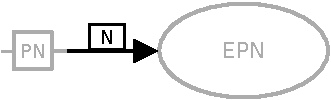
\includegraphics{images/production}
  \caption{The \PD glyph for \glyph{production}.}
  \label{fig:production}
\end{figure}

A cardinality label may be associated with a \glyph{production} arc, indicating the stoichiometry of a process.

\fig{prod-card} illustrates the use of \corr{consumption/production}{\glyph{consumption}/\glyph{production}} arc cardinality labels to represent the stoichiometry of a process.

\begin{figure}[H]
  \centering
  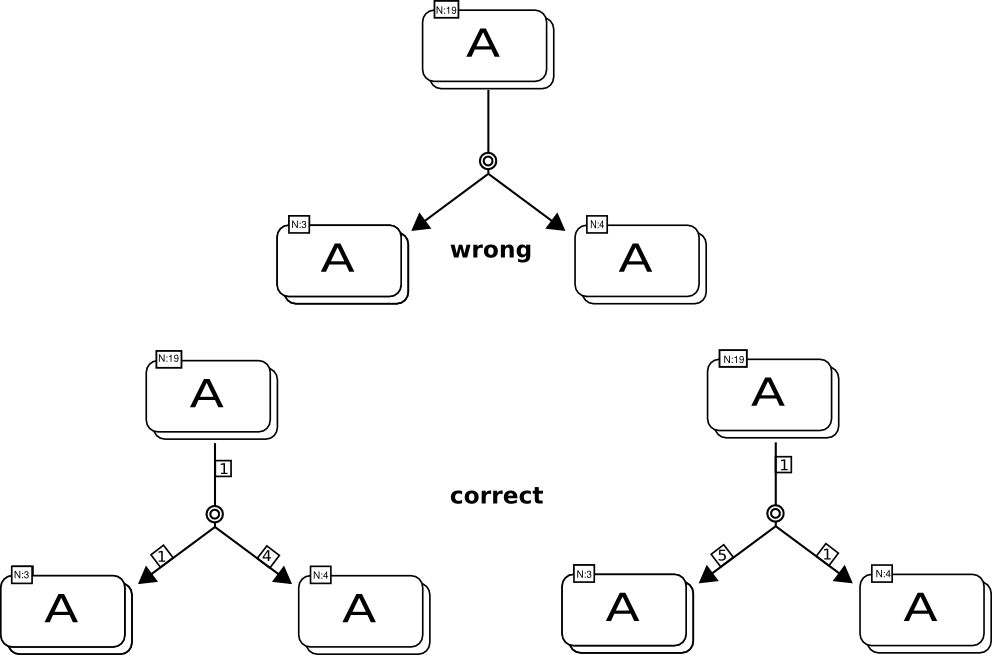
\includegraphics[scale = 0.6]{examples/stoichEx1}
  \caption{Cardinality for production arcs.
  \add{The process on the top is wrong as the stoichiometry is not represented, which leads to ambiguity.}}
  \label{fig:prod-card}
\end{figure}

% The following is for [X]Emacs users.  Please leave in place.
% Local Variables:
% TeX-master: "../sbgn_PD-level1"
% End:
